%! Author = alexis
%! Date = 03/05/2021

% Preamble
\documentclass[12pt]{article}
\title{Initiation à la recherche : \\ Bao-Anh Tran / Deroo Alexis}
\date{2021 - Mai}

% Packages
\usepackage{amsmath}
\usepackage{graphicx}
\usepackage[utf8]{inputenc}
\usepackage[T1]{fontenc}
\usepackage[french]{babel}

% Document
\begin{document}
    \maketitle
    \tableofcontents
    \newpage

    \section{Introduction}\label{sec:introduction}
    
    \newpage
    \section{Ruslan Sadykov}\label{sec:le-chercheur}

    \begin{center}
        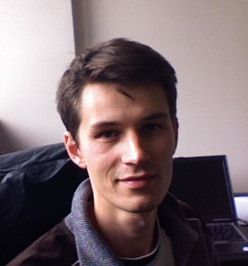
\includegraphics[width=5cm]{image/photo1.jpg}
    \end{center}

    Le professeur Sadykov est originaire de Russie, son domaine de recherche est la recherche opérationnelle. Depuis
    2008 le professeur Sadykov a rejoint l'équipe RealOpt comme membre permanent dans l'équipe. Pour le professeur
    Sadykov, La recherche scientifique permet d'améliorer le préexistant et d'optimiser les couts en temps,
    en ressources, \ldots. C'est cet aspect de la recherche qui lui donne la motivation et la satisfaction dans son
    travail.

    \subsection*{Parcours professionel}\label{subsec:parcours-professionel}

    \begin{itemize}
    \item Etude universitaire en Russie.
    \item Doctorat en Belgique à L'Université catholique de Louvain dans le Centre de recherche opérationnelle et
    d'économétrie.
    Le sujet de sa thèse est: "Integer Programming-based Decomposition Approaches for Solving Machine Scheduling Problems".
    \item Post-Doctorat à l'école Polytechnique de Paris dans l'équipe d'Algorithmie et d'optimisation avec le
    professeur Philippe Baptiste.
    \end{itemize}

    \begin{figure}
        \centering
        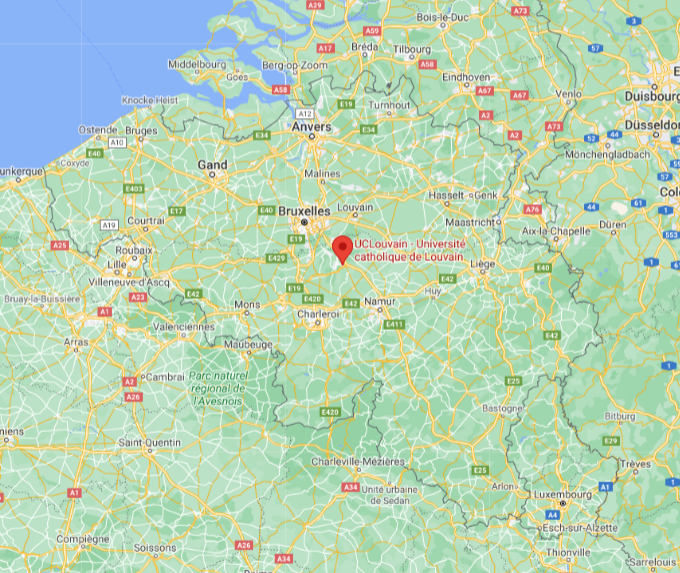
\includegraphics[width=6cm]{image/Map-UCLouvain.png}
        \caption{Université Catholique de Louvain}
        \label{fig:UC Louvain}
    \end{figure}

    \newpage
    \section{RealOPT}\label{sec:realopt}

    L'équipe RealOpt est une équipe de recherche basée à Bordeaux.
    Son domaine de recherche est la recherche opérationnelle.
    le projet vise à développer des formulations et des algorithmes pour des problèmes d'optimisation en exploitant les dernières techniques de reformulation, des outils de programmation non linéaires et des outils de théorie des graphes.
    L'équipe est composé de 6 membres permanents ainsi qu'une dizaine de membres non permanent.
    Les membres permanents sont :
    \begin{itemize}
        \item Francois Clautiaux  (Prof. à l'université de Bordeaux, chef d'équipe à la suite de
        François Vanderbeck)
        \item Boris Detienne (Assist. Prof. à l'université de Bordeaux)
        \item Aurelien Froger (Assist. Prof. à l'université de Bordeaux)
        \item Arnaud Pêcher (Prof. à l'université de Bordeaux)
        \item Pierre Pesneau (Assist. Prof. à l'université de Bordeaux)
        \item Ruslan Sadykov (Chercheur à l'Inria)
    \end{itemize}
    Ce sont des enseignants-chercheurs de l'université de Bordeaux affilié au laboratoire proche de l'université
    dont l'INRIA, le CNRS, \ldots .
    L'équipe est en collaboration avec différents acteurs professionnels pour répondre à certaines problématiques
    d'optimisation.
    Certains de ces acteurs sont EDF, Orange, Saint Gobain ou encore Thalès. Grâce à ces acteurs, l'quipe cible des problèmes à grande échelle notamment dans la conception de réseau, dans la logistique, la planification, les problèmes de découpe et d'emballage, \ldots .
    Après 12 ans de recherches, l'équipe arrive en fin de mission.
    À son terme, l'équipe de chercheurs se renouvellera et changera de nom.

    \section{Le projet de recherche}\label{sec:le-projet-de-recherche}

    \subsection{Amélioriation et optimisation}\label{subsec:amelioriation-et-optimisation}
    Introduction pour expliquer comment sont orientées les différentes pistes de travail
    (besoin des industriels, spécialitée des cherheurs, \ldots)
    \subsection{Deux algorithme, une solution ?}\label{subsec:deux-algorithme,-une-solution-?}
    \subsubsection{Heuristique}
    \subsubsection{Exact}
    \subsubsection{Conclusion}
    \subsection{Un exemple : "Vehicle routing"}\label{subsec:un-exemple-:-"vehicle-routing"}
    \subsection{Conclusion}\label{subsec:conclusion}


    \section{Des perspectives futures ?}\label{sec:des-perspectives-futures-?}


    \section{Conclusion}\label{sec:conclusion}

\end{document}